%%%%%%%%%%%%%%%%%%%%%%%%%%%%%%%%%%%%%%%%%
% Lachaise Assignment
% LaTeX Template
% Version 1.0 (26/6/2018)
%
% This template originates from:
% http://www.LaTeXTemplates.com
%
% Authors:
% Marion Lachaise & François Févotte
% Vel (vel@LaTeXTemplates.com)
%
% License:
% CC BY-NC-SA 3.0 (http://creativecommons.org/licenses/by-nc-sa/3.0/)
% 
%%%%%%%%%%%%%%%%%%%%%%%%%%%%%%%%%%%%%%%%%

%----------------------------------------------------------------------------------------
%	PACKAGES AND OTHER DOCUMENT CONFIGURATIONS
%----------------------------------------------------------------------------------------

\documentclass{article}

%%%%%%%%%%%%%%%%%%%%%%%%%%%%%%%%%%%%%%%%%
% Lachaise Assignment
% Structure Specification File
% Version 1.0 (26/6/2018)
%
% This template originates from:
% http://www.LaTeXTemplates.com
%
% Authors:
% Marion Lachaise & François Févotte
% Vel (vel@LaTeXTemplates.com)
%
% License:
% CC BY-NC-SA 3.0 (http://creativecommons.org/licenses/by-nc-sa/3.0/)
% 
%%%%%%%%%%%%%%%%%%%%%%%%%%%%%%%%%%%%%%%%%

%----------------------------------------------------------------------------------------
%	PACKAGES AND OTHER DOCUMENT CONFIGURATIONS
%----------------------------------------------------------------------------------------

\usepackage{amsmath,amsfonts,stmaryrd,amssymb} % Math packages

\usepackage{enumerate} % Custom item numbers for enumerations

\usepackage[ruled]{algorithm2e} % Algorithms

\usepackage[framemethod=tikz]{mdframed} % Allows defining custom boxed/framed environments

\usepackage{listings} % File listings, with syntax highlighting
\lstset{
	basicstyle=\ttfamily, % Typeset listings in monospace font
}

%----------------------------------------------------------------------------------------
%	DOCUMENT MARGINS
%----------------------------------------------------------------------------------------

\usepackage{geometry} % Required for adjusting page dimensions and margins

\geometry{
	paper=a4paper, % Paper size, change to letterpaper for US letter size
	top=2.5cm, % Top margin
	bottom=3cm, % Bottom margin
	left=2.5cm, % Left margin
	right=2.5cm, % Right margin
	headheight=14pt, % Header height
	footskip=1.5cm, % Space from the bottom margin to the baseline of the footer
	headsep=1.2cm, % Space from the top margin to the baseline of the header
	%showframe, % Uncomment to show how the type block is set on the page
}

%----------------------------------------------------------------------------------------
%	FONTS
%----------------------------------------------------------------------------------------

\usepackage[utf8]{inputenc} % Required for inputting international characters
\usepackage[T1]{fontenc} % Output font encoding for international characters
\usepackage[babel]{} % Output font encoding for international characters

\usepackage{XCharter} % Use the XCharter fonts

%----------------------------------------------------------------------------------------
%	COMMAND LINE ENVIRONMENT
%----------------------------------------------------------------------------------------

% Usage:
% \begin{commandline}
%	\begin{verbatim}
%		$ ls
%		
%		Applications	Desktop	...
%	\end{verbatim}
% \end{commandline}

\mdfdefinestyle{commandline}{
	leftmargin=10pt,
	rightmargin=10pt,
	innerleftmargin=15pt,
	middlelinecolor=black!50!white,
	middlelinewidth=2pt,
	frametitlerule=false,
	backgroundcolor=black!5!white,
	frametitle={Command Line},
	frametitlefont={\normalfont\sffamily\color{white}\hspace{-1em}},
	frametitlebackgroundcolor=black!50!white,
	nobreak,
}

% Define a custom environment for command-line snapshots
\newenvironment{commandline}{
	\medskip
	\begin{mdframed}[style=commandline]
}{
	\end{mdframed}
	\medskip
}

%----------------------------------------------------------------------------------------
%	FILE CONTENTS ENVIRONMENT
%----------------------------------------------------------------------------------------

% Usage:
% \begin{file}[optional filename, defaults to "File"]
%	File contents, for example, with a listings environment
% \end{file}

\mdfdefinestyle{file}{
	innertopmargin=1.6\baselineskip,
	innerbottommargin=0.8\baselineskip,
	topline=false, bottomline=false,
	leftline=false, rightline=false,
	leftmargin=2cm,
	rightmargin=2cm,
	singleextra={%
		\draw[fill=black!10!white](P)++(0,-1.2em)rectangle(P-|O);
		\node[anchor=north west]
		at(P-|O){\ttfamily\mdfilename};
		%
		\def\l{3em}
		\draw(O-|P)++(-\l,0)--++(\l,\l)--(P)--(P-|O)--(O)--cycle;
		\draw(O-|P)++(-\l,0)--++(0,\l)--++(\l,0);
	},
	nobreak,
}

% Define a custom environment for file contents
\newenvironment{file}[1][File]{ % Set the default filename to "File"
	\medskip
	\newcommand{\mdfilename}{#1}
	\begin{mdframed}[style=file]
}{
	\end{mdframed}
	\medskip
}

%----------------------------------------------------------------------------------------
%	NUMBERED QUESTIONS ENVIRONMENT
%----------------------------------------------------------------------------------------

% Usage:
% \begin{question}[optional title]
%	Question contents
% \end{question}

\mdfdefinestyle{question}{
	innertopmargin=1.2\baselineskip,
	innerbottommargin=0.8\baselineskip,
	roundcorner=5pt,
	nobreak,
	singleextra={%
		\draw(P-|O)node[xshift=1em,anchor=west,fill=white,draw,rounded corners=5pt]{%
		Question \theQuestion\questionTitle};
	},
}

\newcounter{Question} % Stores the current question number that gets iterated with each new question

% Define a custom environment for numbered questions
\newenvironment{question}[1][\unskip]{
	\bigskip
	\stepcounter{Question}
	\newcommand{\questionTitle}{~#1}
	\begin{mdframed}[style=question]
}{
	\end{mdframed}
	\medskip
}

%----------------------------------------------------------------------------------------
%	WARNING TEXT ENVIRONMENT
%----------------------------------------------------------------------------------------

% Usage:
% \begin{warn}[optional title, defaults to "Warning:"]
%	Contents
% \end{warn}

\mdfdefinestyle{warning}{
	topline=false, bottomline=false,
	leftline=false, rightline=false,
	nobreak,
	singleextra={%
		\draw(P-|O)++(-0.5em,0)node(tmp1){};
		\draw(P-|O)++(0.5em,0)node(tmp2){};
		\fill[black,rotate around={45:(P-|O)}](tmp1)rectangle(tmp2);
		\node at(P-|O){\color{white}\scriptsize\bf !};
		\draw[very thick](P-|O)++(0,-1em)--(O);%--(O-|P);
	}
}

% Define a custom environment for warning text
\newenvironment{warn}[1][Warning:]{ % Set the default warning to "Warning:"
	\medskip
	\begin{mdframed}[style=warning]
		\noindent{\textbf{#1}}
}{
	\end{mdframed}
}

%----------------------------------------------------------------------------------------
%	INFORMATION ENVIRONMENT
%----------------------------------------------------------------------------------------

% Usage:
% \begin{info}[optional title, defaults to "Info:"]
% 	contents
% 	\end{info}

\mdfdefinestyle{info}{%
	topline=false, bottomline=false,
	leftline=false, rightline=false,
	nobreak,
	singleextra={%
		\fill[black](P-|O)circle[radius=0.4em];
		\node at(P-|O){\color{white}\scriptsize\bf i};
		\draw[very thick](P-|O)++(0,-0.8em)--(O);%--(O-|P);
	}
}

% Define a custom environment for information
\newenvironment{info}[1][Info:]{ % Set the default title to "Info:"
	\medskip
	\begin{mdframed}[style=info]
		\noindent{\textbf{#1}}
}{
	\end{mdframed}
}
 % Include the file specifying the document structure and custom commands

%----------------------------------------------------------------------------------------
%	ASSIGNMENT INFORMATION
%----------------------------------------------------------------------------------------

\title{MAE001: Modelagem Matemática em Finanças I} % Title of the assignment

\author{Ramon Duarte de Melo\\ \texttt{ramonduarte@poli.ufrj.br}} % Author name and email address

\date{Universidade Federal do Rio de Janeiro (UFRJ) --- \today} % University, school and/or department name(s) and a date

%----------------------------------------------------------------------------------------

\begin{document}

\maketitle % Print the title

%----------------------------------------------------------------------------------------
%	INTRODUCTION
%----------------------------------------------------------------------------------------

\section*{Introdução} % Unnumbered section

O objetivo do Projeto I é implementar, avaliar e comparar o algoritmo recursivo proposto pelo livro no capítulo 1.3 e o Método de Monte-Carlo, aplicados à determinação do valor de contratos americanos e europeus de opção de compra e venda, realizando comparações de cunho matemático-estatístico e produzindo gráficos com tais observações. 

Para tal, foi utilizada a linguagem \emph{Python 3.6.7}, com os módulos \emph{numpy} (métodos numéricos) e \emph{matplotlib.pyplot} (visualização de dados).
O programa requer a instalação destes módulos, mas possui uma ferramenta de instalação automatizada das dependências (\emph{pipenv}). 

O código utilizado neste trabalho, bem como o deste relatório e as imagens geradas, foi aberto e disponibilizado publicamente no repositório https://github.com/ramonduarte/mmftrab2.


%----------------------------------------------------------------------------------------
%	PROBLEM 1
%----------------------------------------------------------------------------------------

\section*{Atividade 1} % Numbered section

Nesta atividade, foi implementado o algoritmo sugerido no livro em seu capítulo 1.3.
O procedimento é composto de três etapas:

\begin{enumerate}
	\item obtenção dos valores finais, com especial atenção para evitar a explosão combinatória típica do modelo binomial.
	\item cálculo recursivo dos valores intermediários utilizando os valores finais.
	\item dedução do valor inicial $V_{0}$ do contrato, que também representa seu custo pela teoria de precificação da arbitragem.
\end{enumerate}

Os contratos escolhidos possuem os mesmos parâmetros, tanto para a opção de compra, quanto para a opção de venda:

\begin{itemize}
	\item valor inicial do ativo: 4
	\item taxa de valorização: 100%
	\item taxa de desvalorização: 50%
	\item taxa de renda fixa: 25%
	\item preço de \emph{strike}: 5
\end{itemize}

Estes parâmetros foramutilizados junto às probabilidades neutras a risco $\tilde{p} = \tilde{q} = 0.5$.
Foram calculados os valores para 10 simulações, tais que $N = 2^{k}; k = 1, 2, ..., 10$.



\begin{figure}[]
	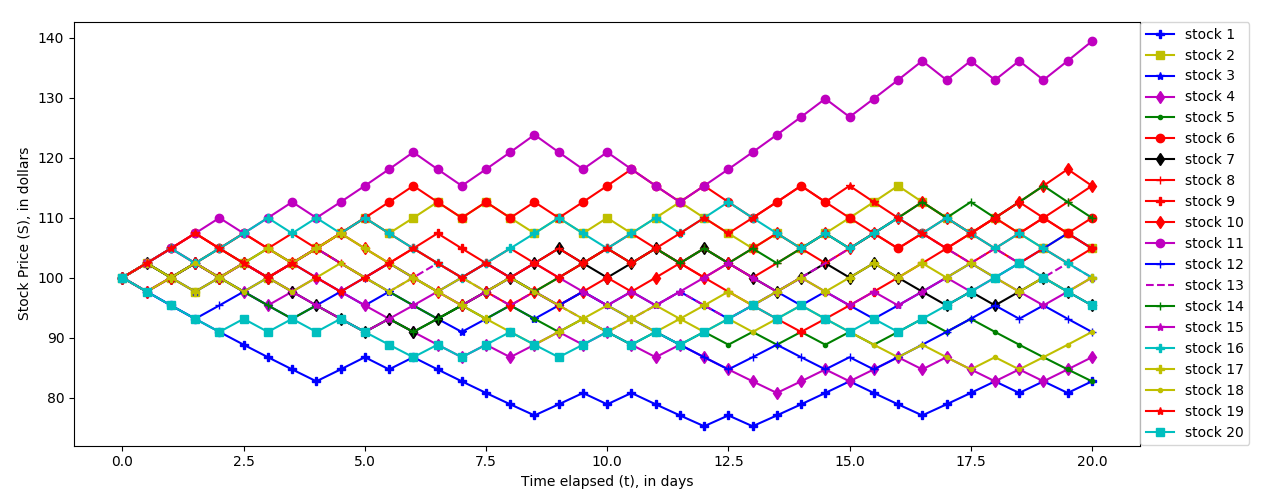
\includegraphics[width=\linewidth]{Figure_1.png}
	\centering
	
	\caption{Passeios aleatórios com $S_{0} = 100$, $u = 1.024$, $d = 1/u = 0.9765625$ e $p = q = 0.5$.}
	\label{}
\end{figure}

%----------------------------------------------------------------------------------------
%	PROBLEM 2
%----------------------------------------------------------------------------------------


\section*{2ª Questão}

Os boxplots foram gerados usando o módulo \emph{matplotlib.pyplot.boxplot}.
Para facilitar a comparação dos boxplots, eles foram agrupados em subplots no mesmo gráfico.
\emph{Outliers} foram marcados com quadrados vermelhos.

\begin{figure}[H]
	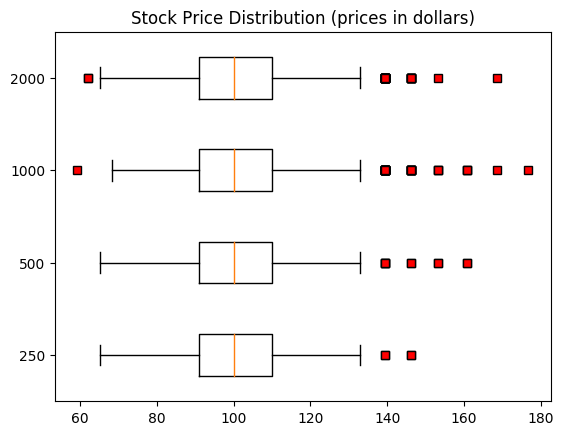
\includegraphics[width=\linewidth]{fig1_250.png}
	\centering
	
	\caption{Boxplots com $250$, $500$, $1000$ e $2000$ iterações, respectivamente, de baixo para cima.}
	\label{}
\end{figure}

%----------------------------------------------------------------------------------------
%	PROBLEM 2
%----------------------------------------------------------------------------------------

\section*{3ª Questão}

Para esta questão, os boxplots foram refeitos utilizando os parâmetros $\Delta t = 0.25$ e $u = 1/d = \sqrt{1.024}$.
Esta configuração gerou uma variância consideravelmente menor, bem como uma quantidade significativamente menor de \emph{outliers}.
Embora todos os ativos pudessem atingir as mesmas taxas de crescimento e decrescimento que no cenário anterior - apesar das taxas serem menores, o maior número de iterações compensa proporcionalmente a redução -, foram raros os ativos que obtiveram mais de 30\% de variação, um cenário bastante comum na segunda questão.

Este fenômeno foi observado porque, como $E[\bar{S}] = E[S_{0}]$ e $E[S(n)] = E[S(n+1)]$, um número maior de repetições tende a aproximar os resultados da média.
A redução da variância em distribuições probabilísticas por conta da ampliação do espaço amostral é bastante conhecida e documentada. 

\begin{figure}[H]
	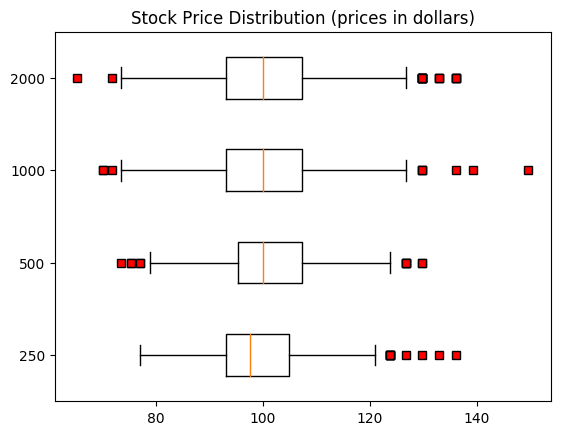
\includegraphics[width=\linewidth]{fig3_250.png}
	\centering
	
	\caption{Boxplots com $250$, $500$, $1000$ e $2000$ iterações, respectivamente, de baixo para cima.}
	\label{}
\end{figure}


%----------------------------------------------------------------------------------------
%	PROBLEM 2
%----------------------------------------------------------------------------------------

\section*{4ª Questão}

O valor esperado de crescimento dos ativos com estes parâmetros é zero, isto é, $E[S(n)] = E[S(n+1)]$.
Portanto, o valor esperado para a média é o mesmo que o inicial do ativo: $E[\bar{S}] = E[S_{0}]$.

Os resultados obtidos convergem fortemente para o previsto na teoria.
A maior variação da média dos passeios aleatórios foi inferior a 3\%, no boxplot $n = 250$ da terceira questão.

%----------------------------------------------------------------------------------------


%----------------------------------------------------------------------------------------
%	PROBLEM 2
%----------------------------------------------------------------------------------------

\section*{5ª Questão}

Para esta questão, algumas adaptações fizeram-se necessárias, haja vista os parâmetros selecionados inicialmente.
Em primeiro lugar, o uso da escala logarítmica aqui dificultaria a visualização dos dados, já que a média, as probabilidades e as taxas foram selecionadas de forma a facilitar a visualização em escala linear.
Em segundo lugar, foi calculado o erro quadrático médio em vez do módulo do erro médio.
Na prática, isto não faz nenhuma diferença, exceto que o gráfico observado será uma parábola em vez de uma reta.

Ao contrário do esperado, o erro quadrático médio cresceu com o aumento da distribuição, embora o aumento tenha sido muito reduzido para ser considerado significativo. 
É provável que este tenha sido um \emph{outlier} em termos de simulação. 
Pode indicar, ainda, um viés na ferramenta de seleção pseudoaleatória utilizada para implementar a rotina \emph{Random}.


\begin{figure}[H]
	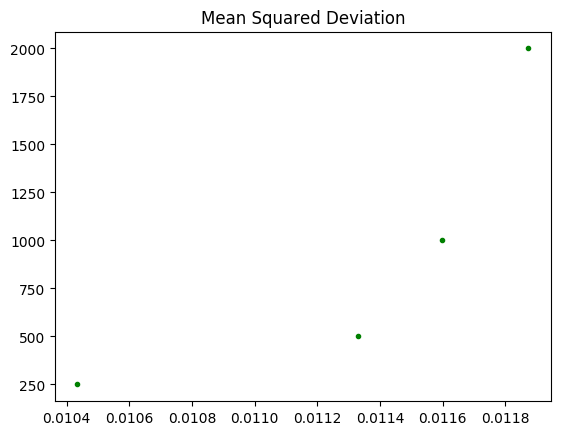
\includegraphics[width=\linewidth]{fig7_250.png}
	\centering
	
	\caption{Erro quadrático médio encontrado com $250$, $500$, $1000$ e $2000$ iterações, respectivamente, de baixo para cima.}
	\label{}
\end{figure}

%----------------------------------------------------------------------------------------


\end{document}
